% =====================================================================
%  Flu forecasting with an SIRS model -- working paper and project log
%  Author: Bernard Frimpong
%
%  This file grows with the project. Each stage adds to it:
%    - the paper sections (Introduction ... Discussion), and
%    - the Project Log appendix (goals, progress, decisions, to-dos).
%  Blue boxes = notes to ourselves; they are removed before submission.
%
%  Compile (from the paper/ folder):
%      pdflatex main
%      bibtex   main
%      pdflatex main
%      pdflatex main
%  or simply upload main.tex, references.bib and the figures to Overleaf.
% =====================================================================
\documentclass[11pt]{article}

\usepackage[margin=1in]{geometry}
\usepackage[T1]{fontenc}
\usepackage{lmodern}
\usepackage{amsmath, amssymb}
\usepackage{graphicx}
\usepackage{booktabs}
\usepackage{float}
\usepackage{array}
\usepackage{enumitem}
\usepackage[table]{xcolor}
\usepackage[most]{tcolorbox}
\usepackage[round]{natbib}
\usepackage[colorlinks=true, linkcolor=blue!50!black, citecolor=blue!50!black,
            urlcolor=blue!50!black]{hyperref}

% Figures live in the repository's results/ folder, one level up.
% (On Overleaf, upload the PNG files next to main.tex; this line still works.)
\graphicspath{{../results/}{./}}

% A blue "note to self" box: what we are doing, decisions, open questions.
\newtcolorbox{note}[1][]{colback=blue!4, colframe=blue!45!black, boxrule=0.5pt,
  arc=2pt, left=6pt, right=6pt, top=4pt, bottom=4pt, fonttitle=\bfseries, title=#1}

% Placeholder for numbers that only exist at the end of the season.
\newcommand{\tbd}[1]{\textcolor{red!70!black}{[#1]}}

\title{Does Mechanism Help? A Prospective Evaluation of a Compartmental SIRS Model
       Against Statistical Baselines in the CDC FluSight 2026--27 Challenge\\[4pt]
       \large Working draft and project log}
\author{Bernard Frimpong\\
        \small Independent researcher (M.S.\ Applied Mathematics, University of Akron)\\
        \small \texttt{bernardfrimpong040@gmail.com}}
\date{Draft updated: 20 October 2026 \quad (Stage 1 complete)}

\begin{document}
\maketitle

% ---------------------------------------------------------------------
\begin{note}[Project status at a glance]
\textbf{Goal.} Compete in CDC FluSight 2026--27 every week (7 Oct 2026 -- 26 May 2027)
with models of increasing structure, then publish a season-long comparison.

\textbf{Current stage.} Stage 1 complete: data pipeline, flat baseline model,
submission validator and a backtest on the 2025--26 season.

\textbf{Next.} First live submission (reference date 24 October 2026, due Wednesday
21 October, 11 PM Eastern); then Stage 2, a statistical growth model.

\textbf{Repository.} \url{https://github.com/bernardfrimpong040-pixel/flu-forecasting-sirs}
\end{note}

% ---------------------------------------------------------------------
\begin{abstract}
Influenza causes tens of thousands of hospital admissions in the United States each
season, and short-term forecasts of those admissions help hospitals and public health
agencies plan. The CDC's FluSight challenge collects weekly probabilistic forecasts of
laboratory-confirmed influenza hospital admissions for every state from dozens of
modelling teams. We ask whether a mechanistic susceptible--infected--recovered--susceptible
(SIRS) model, which represents how an epidemic grows and burns out, forecasts these
admissions better than statistical models that only extrapolate recent data, and in
which phase of the epidemic any advantage appears. All forecasts were submitted to the
FluSight hub in real time during the 2026--27 season, before the outcomes were known.
\tbd{Results: relative weighted interval score of the SIRS model versus the baseline,
overall and by epidemic phase; prediction-interval coverage; conclusion.}
\end{abstract}

% =====================================================================
\section{Introduction}
\label{sec:intro}

Seasonal influenza places a heavy, variable load on hospitals. In the United States,
weekly laboratory-confirmed influenza admissions peaked at 55{,}544 in the 2024--25
season and 42{,}500 in 2025--26 (Section~\ref{sec:data}). Because season timing and
size change from year to year, short-term forecasts one to four weeks ahead are a
practical planning tool.

Since the 2013--14 season the CDC has run FluSight, a collaborative forecasting
challenge in which teams submit forecasts in a common format and are evaluated against
the same data \citep{reich2019, mathis2024}. Models range from statistical time-series
methods to mechanistic compartmental models descended from the work of
\citet{kermack1927}, some combined with data assimilation \citep{shaman2012}.

Comparisons between model families are often made retrospectively, where choices can be
tuned, even unintentionally, to outcomes that are already known. This study is
\emph{prospective}: every forecast was timestamped in the public FluSight repository
before the data it predicts were released.

\paragraph{Research question.}
Across a full season of real-time forecasts, does a mechanistic SIRS model forecast
state-level influenza hospital admissions more accurately than statistical models, and
does any advantage depend on the phase of the epidemic (growth, peak, decline)?

\paragraph{Contributions.}
\begin{enumerate}[nosep]
  \item A transparent, open-source forecasting pipeline submitted weekly to FluSight
        2026--27.
  \item A sequence of models of increasing structure, from a flat baseline to an SIRS
        model with time-varying transmission, evaluated on identical weeks.
  \item An evaluation stratified by epidemic phase and jurisdiction size.
\end{enumerate}

% =====================================================================
\section{Data}
\label{sec:data}

\paragraph{Target.} The forecast target is the weekly number of laboratory-confirmed
influenza hospital admissions reported to the National Healthcare Safety Network
(NHSN) \citep{nhsn2026}, as published in the FluSight hub's \texttt{target-data}
folder \citep{flusighthub2026}. Weeks are CDC epidemiological weeks (Sunday--Saturday)
and are labelled by their final Saturday. The data cover 53 jurisdictions (the 50
states, the District of Columbia, Puerto Rico and the national total) from the week
ending 5 February 2022. Three states have gaps in 2024 (Massachusetts and Minnesota,
May--October; West Virginia, September--October); those weeks are excluded.

\paragraph{Reporting revisions.} Recent weeks can be revised as late reports arrive.
To evaluate forecasts against the information actually available at the time, a dated
snapshot of the target data is saved every time it is downloaded.

\paragraph{Season 2026--27 so far.} National weekly admissions rose from 1{,}247 in
the week ending 5 September 2026 to 3{,}835 in the week ending 10 October 2026, an
earlier start than recent seasons (Figure~\ref{fig:seasons}). In California and
Florida, admissions in week 10 of the season were roughly three to five times their
level at the same point of 2025--26.

\begin{figure}[H]
  \centering
  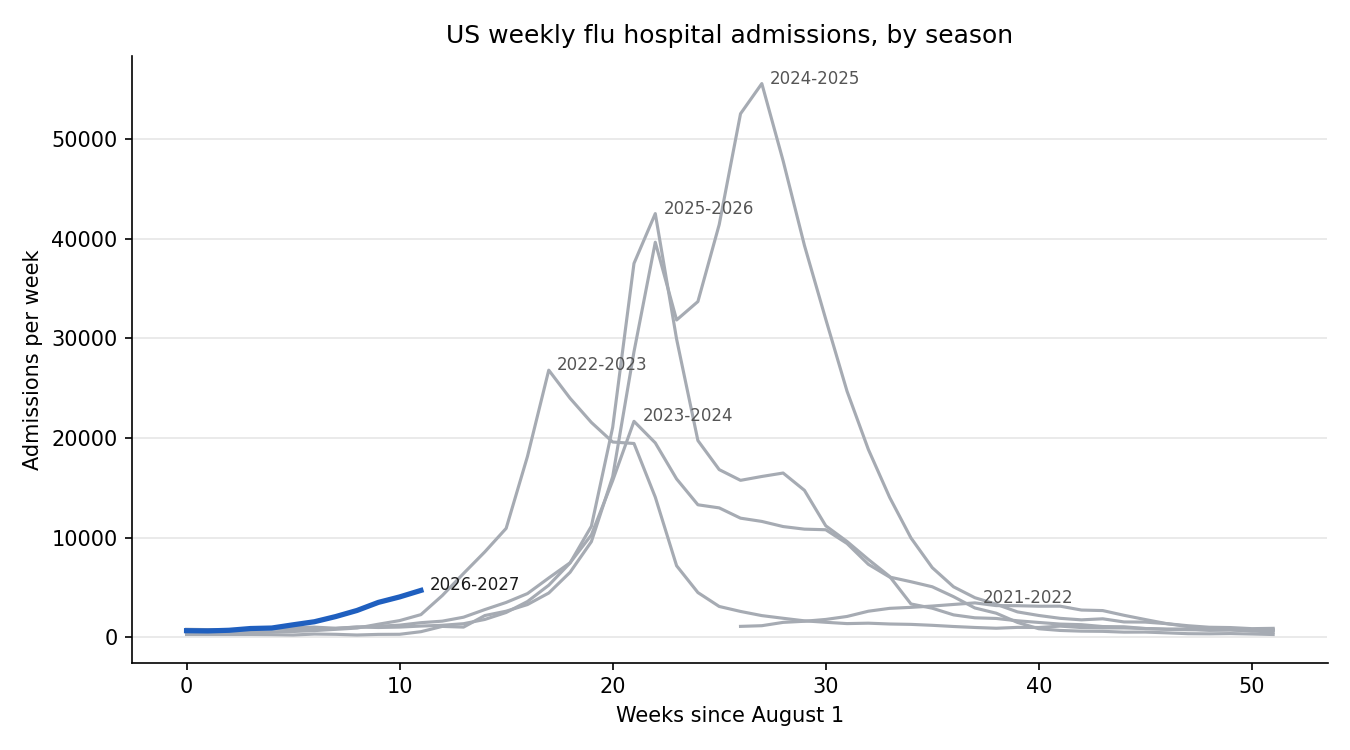
\includegraphics[width=0.85\linewidth]{01_national_seasons.png}
  \caption{US weekly laboratory-confirmed influenza hospital admissions by season,
  aligned by weeks since 1 August. The current season (2026--27) is shown in blue.}
  \label{fig:seasons}
\end{figure}

\begin{table}[ht]
  \centering
  \caption{National peak weekly admissions by season.}
  \label{tab:peaks}
  \begin{tabular}{lrr}
    \toprule
    Season & Peak week ending & Peak admissions \\
    \midrule
    2022--23 & 3 Dec 2022  & 26{,}795 \\
    2023--24 & 30 Dec 2023 & 21{,}662 \\
    2024--25 & 8 Feb 2025  & 55{,}544 \\
    2025--26 & 3 Jan 2026  & 42{,}500 \\
    2026--27 & \multicolumn{2}{c}{\textit{in progress}} \\
    \bottomrule
  \end{tabular}
\end{table}

% =====================================================================
\section{Forecasting task}
\label{sec:task}

Each Wednesday, teams submit forecasts for the epidemiological week ending on the
following Saturday (the \emph{reference date}, horizon $h=0$) and the three weeks after
it ($h=1,2,3$). The newest data available on Wednesday end one week before the reference
date, so a forecast at horizon $h$ is made $k = h+1$ weeks after the last observation.
Forecasts are 23 quantiles of the predictive distribution at levels
\[
  \tau \in \{0.01,\ 0.025,\ 0.05,\ 0.10,\ 0.15,\ \ldots,\ 0.90,\ 0.95,\ 0.975,\ 0.99\},
\]
and admission counts must be whole numbers.

% =====================================================================
\section{Methods}
\label{sec:methods}

\subsection{Stage 1: flat log-scale baseline}
\label{sec:baseline}

Let $y_t$ be weekly admissions in one jurisdiction and $z_t = \log(y_t + 1)$. The
logarithm puts proportional changes on a common scale (a rise from 100 to 120 and from
1{,}000 to 1{,}200 are equal), and the $+1$ handles weeks with zero admissions.

The one-week changes $d_t = z_t - z_{t-1}$ are collected for all pairs of consecutive
weeks (exactly seven days apart) in the previous 156 weeks, restricted to in-season
months (October--May). Each change is also included with its sign reversed, giving a
symmetric set $D = \{d_t\} \cup \{-d_t\}$, so the forecast median equals the last
observation. Let $\hat q_\tau$ be the empirical $\tau$-quantile of $D$.

For a target $k$ weeks after the last observation $y_T$, the forecast quantile is
\begin{equation}
  \hat y_{T+k}(\tau) \;=\; \max\!\Big(0,\ \operatorname{round}\!\big(
      \exp\!\big(z_T + \sqrt{k}\,\hat q_\tau\big) - 1\big)\Big).
  \label{eq:baseline}
\end{equation}
The factor $\sqrt{k}$ comes from treating $z_t$ as a random walk: if weekly changes are
independent with variance $\sigma^2$, the change over $k$ weeks has variance $k\sigma^2$
and standard deviation $\sqrt{k}\,\sigma$. Jurisdictions are modelled independently.

\begin{note}[Planned methods (to be written as each stage is built)]
\begin{itemize}[nosep]
  \item \textbf{Stage 2} -- statistical growth model: regression on recent $z_t$ to
        estimate the current growth rate.
  \item \textbf{Stage 3} -- SIRS model, fitted per jurisdiction:
  \[
    \frac{dS}{dt} = -\beta(t)\frac{SI}{N} + \omega R,\qquad
    \frac{dI}{dt} = \beta(t)\frac{SI}{N} - \gamma I,\qquad
    \frac{dR}{dt} = \gamma I - \omega R,
  \]
  with hospital admissions modelled as a fitted fraction of new infections.
  \item \textbf{Stage 4} -- uncertainty from an ensemble of fitted parameter sets or a
        particle filter.
  \item \textbf{Stage 5} (stretch) -- hybrid: SIRS plus a learned error correction.
\end{itemize}
\end{note}

% =====================================================================
\section{Evaluation}
\label{sec:evaluation}

\paragraph{Weighted interval score.} Following \citet{bracher2021}, a forecast given by
quantiles $x_\tau$ at the level set $\mathcal{T}$ (with $|\mathcal{T}| = 23$ and the
median included) is scored against the observed value $y$ by
\begin{equation}
  \mathrm{WIS}(x, y) \;=\; \frac{2}{|\mathcal{T}|}\sum_{\tau\in\mathcal{T}}
     \big(\mathbf{1}\{y < x_\tau\} - \tau\big)\,(x_\tau - y),
  \label{eq:wis}
\end{equation}
the average quantile (pinball) loss, which is a proper scoring rule
\citep{gneiting2007}. Lower is better. WIS rewards forecasts that are both close to the
truth and no wider than necessary.

\paragraph{Coverage.} The empirical coverage of the central 50\% and 95\% prediction
intervals (between the 0.25 and 0.75, and the 0.025 and 0.975 quantiles). A
well-calibrated forecaster achieves about 0.50 and 0.95.

\paragraph{Relative skill.} \tbd{Season results will be reported as relative WIS
versus the FluSight baseline and ensemble, by horizon, by epidemic phase (growth, peak,
decline) and by jurisdiction size.}

% =====================================================================
\section{Results}
\label{sec:results}

\subsection{Retrospective check of the baseline on the 2025--26 season}

Before the live season, the baseline (Section~\ref{sec:baseline}) was run for each of
the 34 Saturdays from 11 October 2025 to 30 May 2026 using only data dated before each
reference week, and scored against the later observations (Table~\ref{tab:backtest}).

\begin{table}[ht]
  \centering
  \caption{Baseline backtest on the 2025--26 season. WIS is in admissions per week;
  ``States'' averages over 52 jurisdictions. Ideal coverage is 0.50 and 0.95.}
  \label{tab:backtest}
  \begin{tabular}{llrrr}
    \toprule
    Level & Horizon (weeks after last data) & Mean WIS & 50\% coverage & 95\% coverage \\
    \midrule
    States & 0 (1) & 36.3  & 0.53 & 0.96 \\
    States & 1 (2) & 66.3  & 0.46 & 0.94 \\
    States & 2 (3) & 92.3  & 0.43 & 0.91 \\
    States & 3 (4) & 114.0 & 0.40 & 0.89 \\
    \midrule
    US     & 0 (1) & 1{,}601.8 & 0.56 & 0.91 \\
    US     & 1 (2) & 3{,}170.7 & 0.44 & 0.91 \\
    US     & 2 (3) & 4{,}453.1 & 0.32 & 0.74 \\
    US     & 3 (4) & 5{,}450.1 & 0.29 & 0.74 \\
    \bottomrule
  \end{tabular}
\end{table}

Two patterns stand out. First, one week ahead the intervals are close to nominal
coverage, but coverage falls with horizon, most sharply for the national series (95\%
coverage of 0.74 at four weeks). The $\sqrt{k}$ scaling in~\eqref{eq:baseline} assumes
independent weekly changes; during an epidemic, a rise this week tends to be followed by
a rise next week, so uncertainty grows faster than $\sqrt{k}$. Second, the flat median
lags every turn of the epidemic by one to two weeks (Figure~\ref{fig:backtest}),
under-predicting the growth phase and over-predicting the decline. A model with
epidemic dynamics should reduce exactly this error; testing whether it does is the
purpose of Stages 2--3.

\begin{figure}[H]
  \centering
  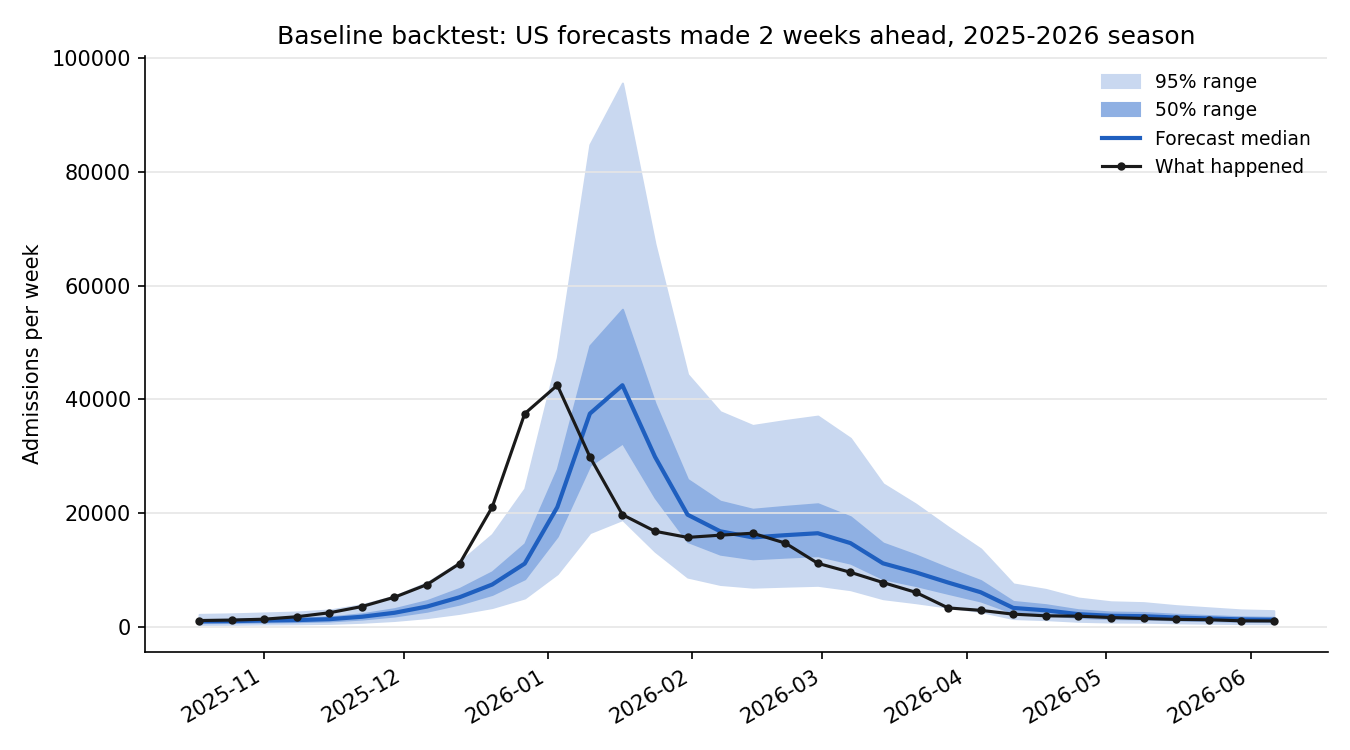
\includegraphics[width=0.85\linewidth]{03_backtest_us_forecasts.png}
  \caption{Baseline forecasts for the US made two weeks after the last observation
  (horizon 1), 2025--26 season: median (line), 50\% and 95\% intervals (bands), and
  observed admissions (black).}
  \label{fig:backtest}
\end{figure}

\paragraph{Limitation of the backtest.} It uses the current, revised data rather than
the data as first reported, so live performance is expected to be somewhat worse.

\subsection{Live season 2026--27}
\tbd{Weekly results to be added as the season progresses.}

% =====================================================================
\section{Discussion}
\label{sec:discussion}
\tbd{To be written after the season: main finding; when mechanism helps or does not;
comparison with other FluSight models; limitations (single season, reporting
revisions, independent jurisdictions); future work.}

% =====================================================================
\section*{Code and data availability}
All code, weekly forecast files and dated data snapshots are available at
\url{https://github.com/bernardfrimpong040-pixel/flu-forecasting-sirs}. Forecasts were
also submitted to the FluSight hub \citep{flusighthub2026}. All data are public,
aggregated counts; no individual-level data were used.

\section*{Use of AI assistance}
Code and draft text were prepared with the help of Claude (Anthropic). The author
reviewed, ran and verified all code, made the modelling decisions, and takes
responsibility for the content.

\bibliographystyle{plainnat}
\bibliography{references}

% =====================================================================
\appendix
\section{Project log}
\label{app:log}

\subsection{Goals}
\begin{enumerate}[nosep]
  \item Submit a valid FluSight forecast every Wednesday from October 2026 to
        26 May 2027.
  \item Build models of increasing structure: baseline $\to$ statistical growth
        $\to$ SIRS $\to$ SIRS with uncertainty $\to$ hybrid.
  \item Post the season evaluation as a medRxiv preprint and submit to a journal
        (June--July 2027).
\end{enumerate}

\subsection{Stage progress}
\begin{center}
\begin{tabular}{>{\raggedright}p{1.6cm} >{\raggedright}p{5.2cm} p{2.4cm} p{4.6cm}}
  \toprule
  Stage & Content & Status & Key outputs \\
  \midrule
  1 & Data pipeline, flat baseline, validator, backtest & Complete (20 Oct 2026) &
      Scripts 01--05; Table~\ref{tab:backtest}; Figures~\ref{fig:seasons},~\ref{fig:backtest} \\
  2 & Statistical growth model & Next & -- \\
  3 & SIRS with time-varying $\beta(t)$ & Planned & -- \\
  4 & Ensemble / particle-filter uncertainty & Planned & -- \\
  5 & Hybrid SIRS + ML correction & Stretch & -- \\
  6 & Season evaluation and paper & June 2027 & -- \\
  \bottomrule
\end{tabular}
\end{center}

\subsection{Decisions and reasons}
\begin{itemize}[nosep]
  \item \textbf{Work on the log scale} -- epidemic changes are proportional.
  \item \textbf{Use only in-season weeks (Oct--May) for the baseline's changes} --
        summer weeks with tiny counts would otherwise distort the spread.
  \item \textbf{Keep dated data snapshots} -- needed to evaluate against the data as it
        was on each forecast day.
  \item \textbf{Submit the baseline as a non-designated reference model} -- it is a
        yardstick, not a contender for the CDC ensemble.
\end{itemize}

\subsection{Open questions}
\begin{itemize}[nosep]
  \item How to define epidemic phases (growth, peak, decline) objectively for the
        stratified evaluation.
  \item Whether to forecast the optional targets (rate-trend category, peak week)
        once the SIRS model is running.
  \item Before posting the preprint: contact \texttt{flusight@cdc.gov} about
        attribution of hub forecast data.
\end{itemize}

\subsection{Weekly submission log}
\begin{center}
\begin{tabular}{llll}
  \toprule
  Reference date & Model(s) submitted & Data through & Notes \\
  \midrule
    24 Oct 2026 & BFrimpong-baseline & 17 Oct 2026 & First submission; PR opened 21 Oct \\
  \bottomrule
\end{tabular}
\end{center}

\end{document}
